\documentclass[twoside]{article}
\setlength{\oddsidemargin}{0.25 in}
\setlength{\evensidemargin}{-0.25 in}
\setlength{\topmargin}{-0.6 in}
\setlength{\textwidth}{6.5 in}
\setlength{\textheight}{8.5 in}
\setlength{\headsep}{0.75 in}
\setlength{\parindent}{0 in}
\setlength{\parskip}{0.1 in}

\usepackage{graphicx}
\usepackage{url}
\usepackage{amsmath}
\usepackage{amssymb}
\usepackage{subcaption}

%
% The following commands sets up the lecnum (lecture number)
% counter and make various numbering schemes work relative
% to the lecture number.
%
\newcounter{lecnum}
\renewcommand{\thepage}{\thelecnum-\arabic{page}}
\renewcommand{\thesection}{\thelecnum.\arabic{section}}
\renewcommand{\theequation}{\thelecnum.\arabic{equation}}
\renewcommand{\thefigure}{\thelecnum.\arabic{figure}}
\renewcommand{\thetable}{\thelecnum.\arabic{table}}
\newcommand{\dnl}{\mbox{}\par}

%
% The following macro is used to generate the header.
%
\newcommand{\lecture}[4]{
  \pagestyle{myheadings}
  \thispagestyle{plain}
  \newpage
  \setcounter{lecnum}{#1}
  \setcounter{page}{1}
  \noindent
  \begin{center}
  \framebox{
     \vbox{\vspace{2mm}
   \hbox to 6.28in { {\bf CMPSCI~590S~~~Systems for Data Science
                       \hfill Fall 2017} }
      \vspace{4mm}
      \hbox to 6.28in { {\Large \hfill Lecture #1  \hfill} }
%       \hbox to 6.28in { {\Large \hfill Lecture #1: #2  \hfill} }
      \vspace{2mm}
      \hbox to 6.28in { {\it Lecturer: #3 \hfill Scribe: #4} }
     \vspace{2mm}}
  }
  \end{center}
  \markboth{Lecture #1: #2}{Lecture #1: #2}
  \vspace*{4mm}
}

%
% Convention for citations is authors' initials followed by the year.
% For example, to cite a paper by Leighton and Maggs you would type
% \cite{LM89}, and to cite a paper by Strassen you would type \cite{S69}.
% (To avoid bibliography problems, for now we redefine the \cite command.)
%
\renewcommand{\cite}[1]{[#1]}

% \input{epsf}

%Use this command for a figure; it puts a figure in wherever you want it.
%usage: \fig{NUMBER}{FIGURE-SIZE}{CAPTION}{FILENAME}
\newcommand{\fig}[4]{
           \vspace{0.2 in}
           \setlength{\epsfxsize}{#2}
           \centerline{\epsfbox{#4}}
           \begin{center}
           Figure \thelecnum.#1:~#3
           \end{center}
   }

% Use these for theorems, lemmas, proofs, etc.
\newtheorem{theorem}{Theorem}[lecnum]
\newtheorem{lemma}[theorem]{Lemma}
\newtheorem{proposition}[theorem]{Proposition}
\newtheorem{claim}[theorem]{Claim}
\newtheorem{corollary}[theorem]{Corollary}
\newtheorem{definition}[theorem]{Definition}
\newenvironment{proof}{{\bf Proof:}}{\hfill\rule{2mm}{2mm}}

% Some useful equation alignment commands, borrowed from TeX
\makeatletter
\def\eqalign#1{\,\vcenter{\openup\jot\m@th
 \ialign{\strut\hfil$\displaystyle{##}$&$\displaystyle{{}##}$\hfil
     \crcr#1\crcr}}\,}
\def\eqalignno#1{\displ@y \tabskip\@centering
 \halign to\displaywidth{\hfil$\displaystyle{##}$\tabskip\z@skip
   &$\displaystyle{{}##}$\hfil\tabskip\@centering
   &\llap{$##$}\tabskip\z@skip\crcr
   #1\crcr}}
\def\leqalignno#1{\displ@y \tabskip\@centering
 \halign to\displaywidth{\hfil$\displaystyle{##}$\tabskip\z@skip
   &$\displaystyle{{}##}$\hfil\tabskip\@centering
   &\kern-\displaywidth\rlap{$##$}\tabskip\displaywidth\crcr
   #1\crcr}}
\makeatother

% **** IF YOU WANT TO DEFINE ADDITIONAL MACROS FOR YOURSELF, PUT THEM HERE:



% Some general latex examples and examples making use of the
% macros follow.

\begin{document}

%FILL IN THE RIGHT INFO.
%\lecture{**LECTURE-NUMBER**}{**DATE**}{**LECTURER**}{**SCRIBE**}
\lecture{4}{September 14}{Emery Berger}{Jayanth Hegde, Nidhi Mundra}

\section{Overview}

The class started with discussion on how multiprocessing is difficult to implement and Dennard scaling is becoming obsolete. The solutions to this problem is: Parallel processing.

\section{Approaches to Performing Parallel Processing} Parallel processing can be performed using two approaches: Shared Memory and Distributed Memory.

The shared memory approach makes use of threads while distributed memory makes use of processes on multiple machines. In case
of the latter, explicit communication mechanisms such as message passing are required. \\
\begin{figure}[h]
\centering
    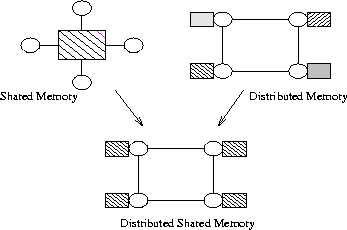
\includegraphics[scale=1]{shared_vs_distributed_memories}
    \caption{Shared memory and Distributed memories}
\end{figure}

Message passing and threads are duals in the sense that thread actions become communication at the hardware level.

\section{Threads vs Processes}

1) Heap is shared amongst various threads while processes do not share the heap.\\
2) Global variables are shared amongst threads while processes do not share them.\\
3) Code is shared in case of both threads and processes.\\
4) Stack variables are not shared in case of both threads and processes.

\section{Race condition} Non-determinism in the access of shared resources between threads. \\
To prevent racing, the ordering of events must be controlled. This can be done in the following ways:

1) \textit{Wait for threads}\\
2) \textit{Synchronization operation}: Prevents concurrency and orders events. A lock/mutex is used for this purpose. A condition variable
can also be used to do this. A condition variable incorporates a signaling along with locking mechanism. A thread can wait over
a condition variable for a resource under use. As soon as the resource becomes available, the waiting thread is signaled to resume
execution by acquiring the resource. In Java, the wait and notify mechanism provides the same functionality. This method can be used
to enforce happens-before relation among events.

\section{Challenges of Multithreading}
1) Correctness: If proper care is not taken, heisenbugs can arise due to inherent non-determinism in multithreaded programs.\\
2) Performance: Ironically, multithreaded programs can perform badly if synchronization is done inappropriately.\\
3) Load imbalance: It is possible to have situations where one thread does more work than the other.

\section{Some Definitions}

1) \textit{Critical Path or Span of computation}: The maximum sequential path of execution in a multithreaded program. Look at figure~\ref{fig:critical_path}.
\begin{figure}[H]
\centering
    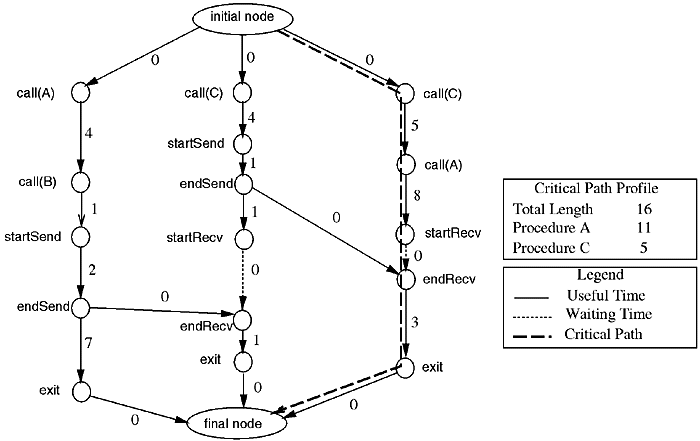
\includegraphics[scale=0.5]{critical_path}
    \caption{Critical Path}
    \label{fig:critical_path}
\end{figure}

2) \textit{Embarrasingly parallel}: A problem that lends itself naturally to parallel processing.

3) \textit{Heisenbug}: A bug that surfaces rarely under certain conditions.

4) \textit{Gustafson's law}: The computation can be scaled in accordance to the scale of the task provided the growth of the problem is comparable to growth in the power of computation.
 Eg: Creating inverted index of webpages.



\end{document}
